
%(BEGIN_QUESTION)
% Copyright 2012, Tony R. Kuphaldt, released under the Creative Commons Attribution License (v 1.0)
% This means you may do almost anything with this work of mine, so long as you give me proper credit

Calculate the operating current through each of the load resistances shown in this circuit (assuming each three-phase load is balanced):

$$\includegraphics[width=15.5cm]{i02119x01.eps}$$

Also, calculate the power dissipated by each load.

\underbar{file i02119}
%(END_QUESTION)





%(BEGIN_ANSWER)

In the direct-connected load, each resistor sees $1 \over \sqrt{3}$ of the 13.8 kV line voltage (7967.4 volts), therefore, each resistor current is equal to:

$$I = {V \over R} = {7967.4 \over 1240} = 6.425 \hbox{ amps}$$

Since each resistor sees 7967.4 volts and carries 6.425 amps, the power for each resistor will be:

$$P = IV = (6.425)(7967.4) = 51.194 \hbox{ kW}$$

The power for this load is simply the power of all resistors combined:  

$$P_{total} = 153.58 \hbox{ kW}$$

\vskip 10pt

The three transformers have their primary windings connected in a Wye configuration, and their secondary windings in a Delta configuration.  Thus, each transformer primary sees 7967.4 volts, stepping it down by a 16.67:1 ratio into 477.95 volts.  The secondary windings, being Delta-connected, make this 477.95 volt value the line voltage for the load.  The load is Delta-connected as well, and so each resistor in that load sees 477.95 volts, giving a resistor current of:

$$I = {V \over R} = {477.95 \over 950} = 0.5031 \hbox{ amps}$$

Since each resistor sees 477.95 volts and carries 0.5031 amp, the power for each resistor will be:

$$P = IV = (0.5031)(477.95) = 240.46 \hbox{ W}$$

The power for this load is simply the power of all resistors combined:  

$$P_{total} = 721.38 \hbox{ W}$$


%(END_ANSWER)





%(BEGIN_NOTES)


%INDEX% Electronics review: 3-phase electrical power 
%INDEX% Electronics review: AC transformer circuit

%(END_NOTES)


